%!TEX TS-program = xelatex
%!TEX encoding = UTF-8 Unicode
% Awesome CV LaTeX Template for CV/Resume
%
% This template has been downloaded from:
% https://github.com/posquit0/Awesome-CV
%
% Author:
% Claud D. Park <posquit0.bj@gmail.com>
% http://www.posquit0.com
%
% Template license:
% CC BY-SA 4.0 (https://creativecommons.org/licenses/by-sa/4.0/)
%


% CONFIGURATIONS
% A4 paper size by default, use 'letterpaper' for US letter
\documentclass[11pt, a4paper]{awesome-cv}

% Configure page margins with geometry
\geometry{left=1.4cm, top=.8cm, right=1.4cm, bottom=1.8cm, footskip=.5cm}

% Specify the location of the included fonts
\fontdir[fonts/]

% Color for highlights
% Awesome Colors: awesome-emerald, awesome-skyblue, awesome-red, awesome-pink, awesome-orange
%                 awesome-nephritis, awesome-concrete, awesome-darknight
\colorlet{awesome}{awesome-skyblue}
% Uncomment if you would like to specify your own color
\definecolor{awesome}{HTML}{0074e8}

% Colors for text
% Uncomment if you would like to specify your own color
% \definecolor{darktext}{HTML}{414141}
% \definecolor{text}{HTML}{333333}
% \definecolor{graytext}{HTML}{5D5D5D}
% \definecolor{lighttext}{HTML}{999999}

% Set false if you don't want to highlight section with awesome color
\setbool{acvSectionColorHighlight}{true}

% If you would like to change the social information separator from a pipe (|) to something else
\renewcommand{\acvHeaderSocialSep}{\quad\textbar\quad}

%	PERSONAL INFORMATION
%	Comment any of the lines below if they are not required
% Available options: circle|rectangle,edge/noedge,left/right
% \photo[rectangle,noedge]{kyle.png}
\name{Kyle W.}{Rader}
\position{Software Engineer{\enskip\cdotp\enskip} Technology Enthusiast}
% \address{}

\mobile{425-241-7977}
\email{kyle@kylerader.ninja}
\homepage{kylerader.ninja}
\github{/kyle-rader}
\linkedin{/in/kylewrader}

% \gitlab{gitlab-id}
% \stackoverflow{SO-id}{SO-name}
% \twitter{@twit}
% \skype{skype-id}
% \reddit{reddit-id}
% \extrainfo{extra informations}

% \quote{`Laughter is the beest medicine."}

\begin{document}

% Print the header with above personal informations
% Give optional argument to change alignment(C: center, L: left, R: right)
\makecvheader

% Print the footer with 3 arguments(<left>, <center>, <right>)
% Leave any of these blank if they are not needed
\makecvfooter
  {\today}
  {Kyle W. Rader}
  {\thepage}

%-------------------------------------------------------------------------------
% Skills
%-------------------------------------------------------------------------------
\cvsection{Skills}
\begin{cvskills}
  \cvskill
    {Current Languages} % Category
    {Ruby, NodeJS, Bash, Python, Cypher (graph query language)} % Skills

  \cvskill
    {Web} % Category
    {Rails, Meteor, Express, React, Ember, HTML, LESS/SASS} % Skills

  \cvskill
    {Tools/Services} % Category
    {Git, Docker, Neo4j, Postgres, MongoDB, Heroku, Joyent/Triton, AWS S3 } % Skills
\end{cvskills}

%-------------------------------------------------------------------------------
% Experience
%-------------------------------------------------------------------------------
\cvsection{Experience}
\begin{cventries}
  \cventry
    {ActionSprout} % Organization
    {Software Engineer} % Job title
    {Redmond/Bellingham, WA} % Location
    {July 2016 - PRESENT $\cdot$ 1 yr 7 mos} % Date(s)
    {
      \begin{cvitems} % Description(s) of tasks/responsibilities
        \item Initiated projects such as Rails micro-service generator, Facebook Graph API RubyGem, usage metrics collection and storage service, content recommendation service, JSON web token authentication standards etc. All of which are used daily.
        \item Pioneered use of Docker/Docker-Compose standardizing developer environments solving the ``works on my machine" problem.
        \item Designed a Neo4j Docker orchestration toolkit for Joyent's Triton platform cutting service costs by over 50\%.
        \item Learned to design micro-services with robust background processing through small, single responsibility, idempotent workers.
      \end{cvitems}
    }
    {
      Tools and training to help nonprofits exceed their goals on Facebook.
    }

  \cventry
    {8las} % Organization
    {Software Development Life Cycle (SDLC) Manager} % Job title
    {Bellingham, WA/Shanghai, China} % Location
    {July 2015 - July 2016 $\cdot$ 1 yr} % Date(s)
    {
      \begin{cvitems} % Description(s) of tasks/responsibilities
        \item Lead and organized 5-6 developers using Git, BitBucket, and agile tracking tools.
        \item In four months moved from a scattered product idea to a beta launch of an AR runtime and SDK codenamed ``Catapult".
        \item Wrote AR demo applications in Unity/C\# using Catapult. Ran and managed live demos for customers and potential investors.
        \item Spent three months in Shanghai after an acqui-hire, integrating development teams and products from Bellingham, WA, Hong Kong, Shanghai, and Chengdu, China. Mission was to build an AR platform on web and mobile technologies.
      \end{cvitems}
    }
    {
      Augmented reality (AR) startup in Bellingham, WA building AR software compatible with the Immy ic60 glasses.
    }

  \cventry
    {Womp Mobile} % Organization
    {Production Engineer} % Job title
    {Bellingham, WA} % Location
    {Mar 2015 - Aug 2015  $\cdot$ 6 mos} % Date(s)
    {
      \begin{cvitems} % Description(s) of tasks/responsibilities
        \item Helped implement a more streamlined development workflow and client project tracking system.
      \end{cvitems}
    }
    {
      Website mobilization by consuming client websites and writing HTML/SASS and Javascript/jQuery to produce a mobile device optimized site.
    }

  \cventry
    {Logos} % Organization
    {Web Developer} % Job title
    {Bellingham, WA} % Location
    {Jun 2013 - Jan 2014  $\cdot$ 8 mos} % Date(s)
    {
      \begin{cvitems} % Description(s) of tasks/responsibilities
        \item Projects inlcuded RabbitMQ message replay, MySQL cluster dashboard, server patch dashboard, and version controlled MySQL schema migration dashboard.
      \end{cvitems}
    }
    {
      Religious study tools, social media, and online publishing. Dev Ops team.
    }

  \cventry
    {Brer Technical} % Organization
    {Software Engineer} % Job title
    {Bellingham, WA} % Location
    {Apr 2012 - Mar 2014  $\cdot$ 2 yrs} % Date(s)
    {
      \begin{cvitems} % Description(s) of tasks/responsibilities
        \item Translated business needs of running a piping test procedure and collecting data into a product definition.
        \item Built Windows desktop application in C\# featuring real-time data collection, visualization, step motor and mega-ohm meter communication.
      \end{cvitems}
    }
    {Industrial fiberglass piping analysis company.}

  \cventry
    {Western Washington University} % Organization
    {Graduate \& Undergraduate Teaching Assistant} % Job title
    {Bellingham, WA} % Location
    {Sept 2011 - Mar 2015  $\cdot$ 3 yrs 6 mos} % Date(s)
    {
      \begin{cvitems} % Description(s) of tasks/responsibilities
        \item Wrote grading scripts for building, compiling, and testing Java programs.
        \item Designed and wrote a new lab sequence in Racket providing students with failing tests for test driven development.
        \item Frequently lectured in labs, ran extended office hours, and maintained excellent student reviews.
      \end{cvitems}
    }
    {Taught Intro to Robotics (C), Programming II \& Linear Data Structures (Java), and Formal Language \& Functional Programming (Lisp/Racket)}

\end{cventries}

\newpage
%-------------------------------------------------------------------------------
% Projects
%-------------------------------------------------------------------------------
\cvsection{Projects}
\begin{cventries}

  \cventry
    {Lead Software Engineer/Co-Founder} % Affiliation/role
    {The Great Puzzle Hunt} % Organization/group
    {https://greatpuzzlehunt.com} % Location
    {June 2015 - PRESENT $\cdot$ 2 yrs 5 mos} % Date(s)
    {
      \begin{cvitems} % Description(s) of tasks/responsibilities
        \item Client application in ReactJS backed by Meteor and Rails API. Deployed on Digital Ocean behind Nginx for forced TLS.
        \item Volunteers scan team QR codes to track puzzle start times. Teams solve and enter puzzle answers in the application.
        \item The web application handles registration/user management, payment web hooks, team formation, ticket redemptions, real-time scoring and game play, and administration tools.
      \end{cvitems}
    }
    {
      Annual event drawing around 500 people to Western Washington University to play in a five-puzzle team scavenger hunt around the campus.
      Teams and volunteers use smartphones to compete on a real-time game platform.
    }

  \cventry
    {Software Engineer/Co-Founder} % Affiliation/role
    {CodeLily Code School} % Organization/group
    {Bellingham, WA} % Location
    {Sept 2014 - Sept 2015 $\cdot$ 1 yr} % Date(s)
    {
      \begin{cvitems} % Description(s) of tasks/responsibilities
        \item Won crowd favorite at Bellingham Pitchfest Feb 2015.
        \item Managed a team of four WWU Computer Science seniors building the CodeLily demo platform (similar to CodePen) with AngularJS and NodeJS/Express.
      \end{cvitems}
    }
    {A Startup Weekend Challenge idea to create a code school with a focus on accessibility for youth and adults switching careers.}

  \cventry
    {Software Engineer} % Affiliation/role
    {Uzility Agile Kanban System} % Organization/group
    {Bellingham, WA} % Location
    {Dec 2013 - Nov 2014 $\cdot$ 11 mos} % Date(s)
    {
      \begin{cvitems} % Description(s) of tasks/responsibilities
        \item Learned agile and scrum methodologies from a certified scrum master.
        \item Migrated code base from CVS to Git.
        \item Developed front and back-end application with HTML, LESS, PHP, MySQL, and jQuery.
      \end{cvitems}
    }
    {Uzility was a web based agile software development tool project.}
\end{cventries}

%-------------------------------------------------------------------------------
% Education
%-------------------------------------------------------------------------------
\cvsection{Education}
\begin{cventries}
  \cventry
  {B.S. Computer Science $\cdot$ 2014} % Degree
  {Western Washington University} % Institution
  {Bellingham, WA} % Location
  {Sept. 2010 - June. 2014} % Date(s)
  {
  \begin{cvitems} % Description(s) bullet points
    \item {2014 Computer Science Dept. Citizenship award}
    \item {2013 Technology Leader of Tomorrow award from Technology Alliance Group NW (TAGNW)}
  \end{cvitems}
  }
  {}

  \cventry
  {M.S. Computer Science $\cdot$ expt 2018} % Degree
  {Western Washington University} % Institution
  {Bellingham, WA} % Location
  {Sept. 2014 - Expt. Spring. 2018} % Date(s)
  {
  \begin{cvitems} % Description(s) bullet points
    \item {Finishing research, part-time, on social media post recommendation system for content curators. In conjunction with ActionSprout.}
    \item {Implemented application features at ActionSprout to collect a dataset of Facebook page-to-post voting observations.}
  \end{cvitems}
  }
  {}

\end{cventries}

\cvsection{Timeline}
\vspace{2mm}

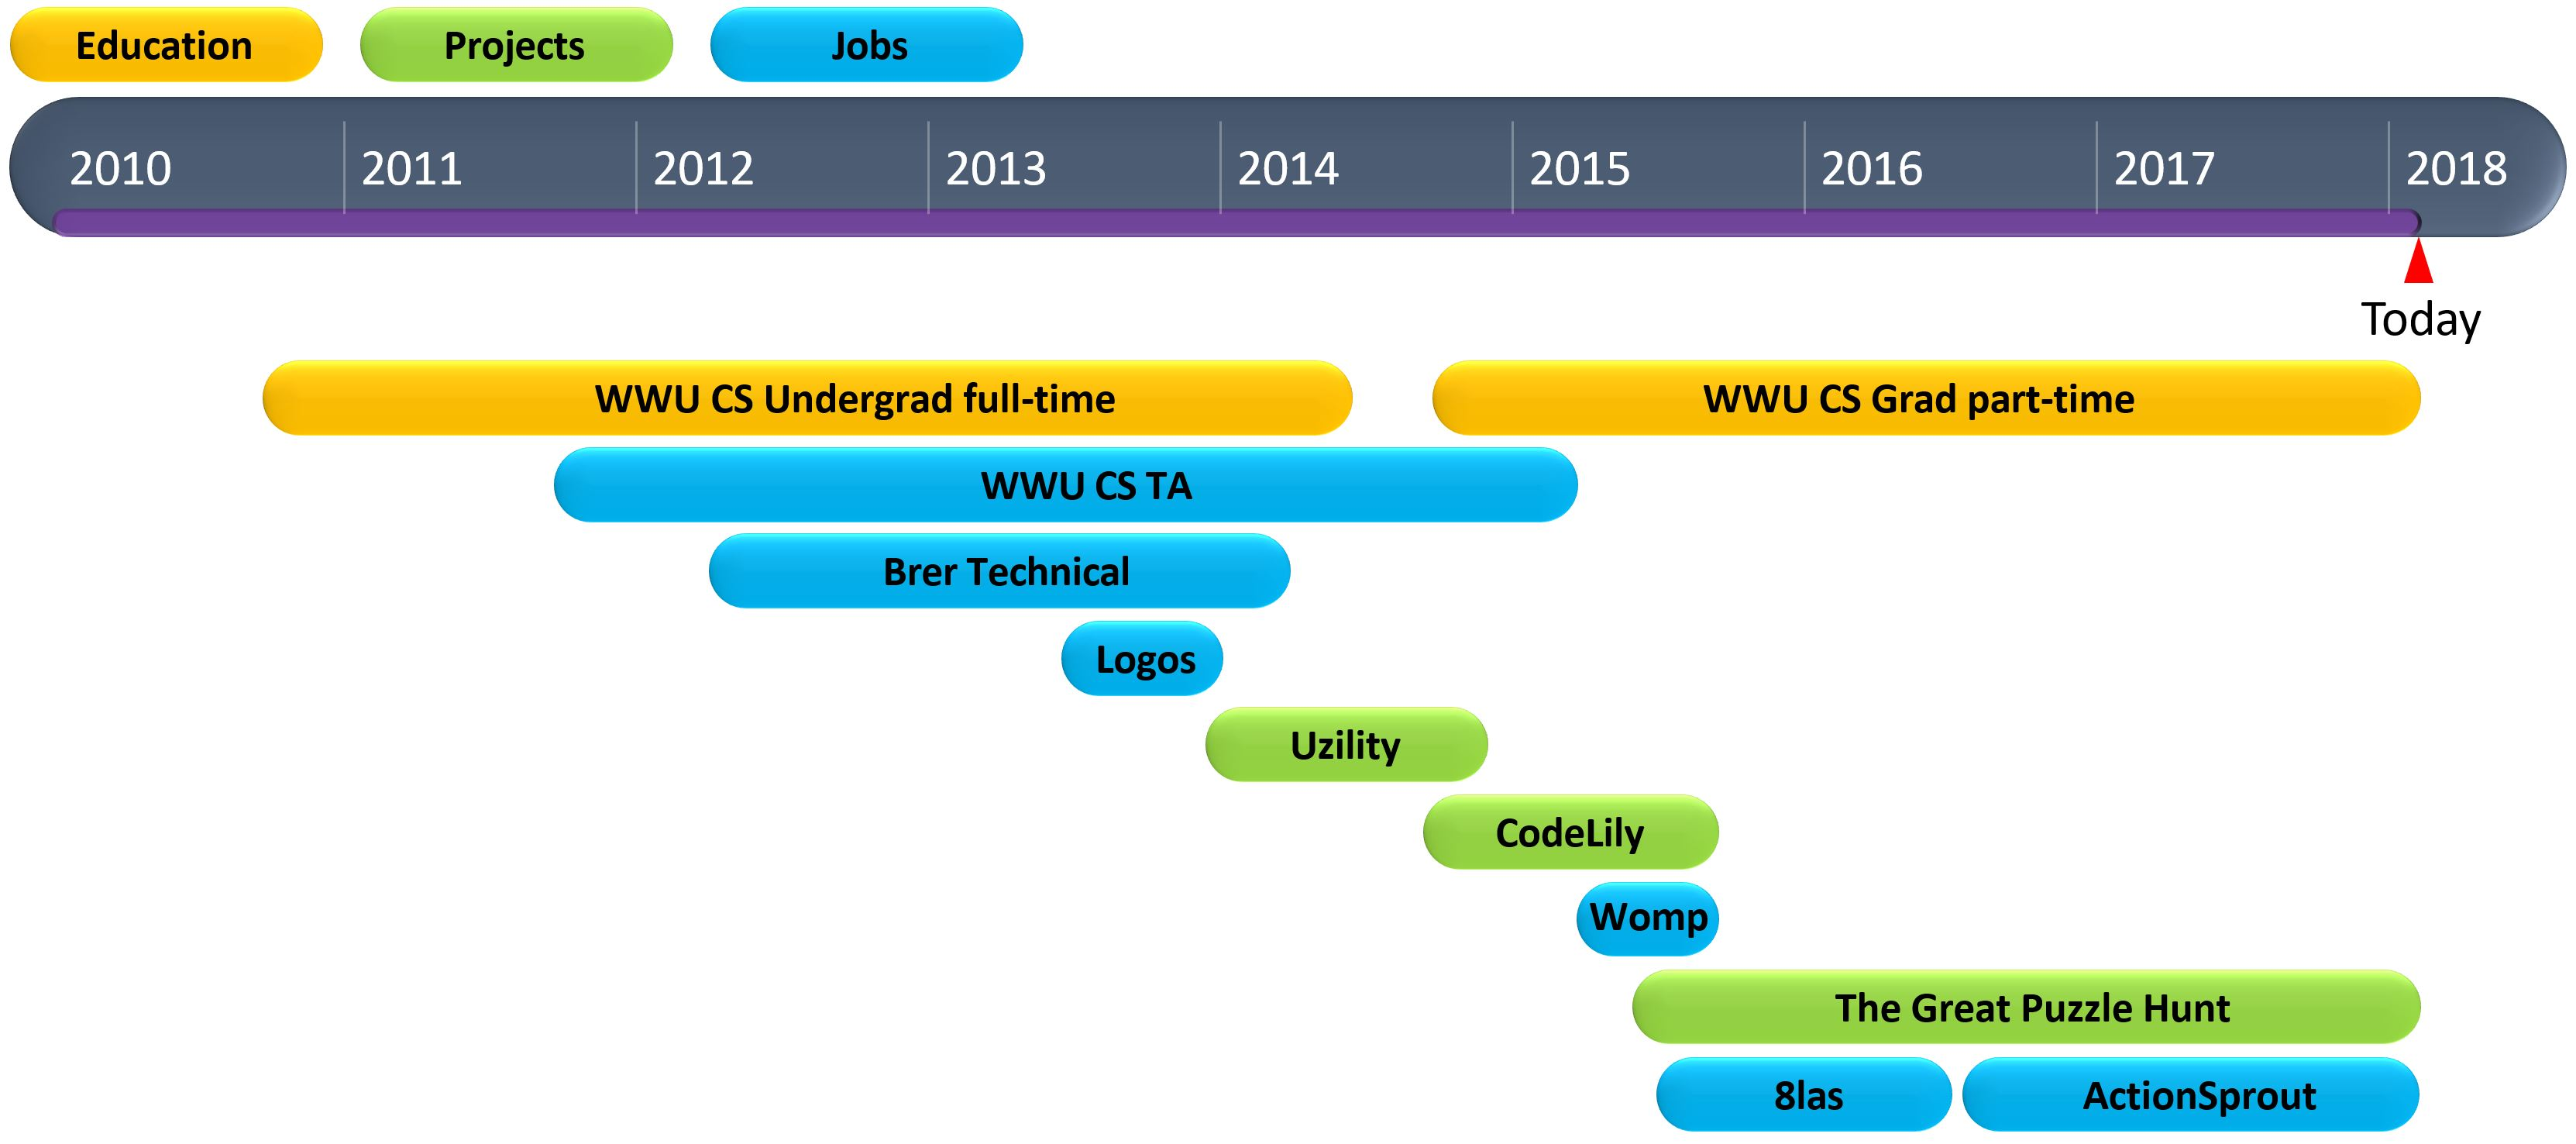
\includegraphics[scale=.3]{kyle_rader_gantt.jpg}

\end{document}
